\section{Introduction}

Although nonlinear systems are difficult to solve analytically, many practical 
systems exhibits regular patterns. 
Those patterns are difficult to be described analytically, but are still 
evident 
enough for human to recognize. 
People are constantly solving nonlinear systems in their daily lift with 
pattern 
recognition, without even realizing them. 
After some training, students learning nonlinear dynamics can make accurate 
predictions of a system's behavior using very limited information. 
For example, we can project the dynamics to a 2D plane, solve the fixed points 
and their locally linear properties, then fill the non linear part with our 
prior knowledge.

On the other hand, recent advances in machine learning and deep neural networks 
show remarkable results in fitting highly non-linear data, e.g., natural 
images, 
and achieves human-level performance. 
A particularly interesting topic is image-to-image translation.
Given enough training data, a neural network can translate images from an input 
domain to an output domain. 
The neural network uses its learned knowledge to fill the missing information, 
such as texture and color, exactly like how we solve nonlinear systems. 
As such, a natural question rises:
Can we train a machine learning model to predict the behavior of some nonlinear 
systems? 

To utilize the successful experience of applying deep neural networks on 
stationary 2D images, in this project, we focus on studying the steady state 
fluid flow around 2D obstacles.  
We craft a set of training images based on conventional computation fluid 
dynamics method, which numerically simulates the fluid using physical models. 
A deep neural network will fit the data and predict steady state velocity field 
around any unseen obstacle shape.  

From our experiments, we find that a deep neural network can accurately predict 
the fluid dynamics in a limited range. 
This machine learning-based approximation approach cannot be as universal as 
conventional simulation methods, but provide a good speedup when dealing with 
repetitive tasks. 
Examples include boat shape optimization, which requires repetitively 
simulating 
the fluid flow around an obstacle, which change little between each 
optimization 
steps. 
As we can easily parallelize the execution of neural network, the neural 
network-based approximation can achieve over 100$\times$ speedup comparing to 
conventional simulations. 

\section{Background}

\subsection{Computational fluid dynamics (CFD)}

Computational fluid dynamics (CFD) is a type of methods that use numerical 
analysis to solve fluid dynamic problems. 
Usually, a fluid field is described using partial differential equations 
(Navier-Stokes equations, the mass and energy conservation equations, the 
turbulence equations, etc.), and then solved using discrete approximations. 

Solving a steady state fluid dynamic problem with CFD generally follows the 
following steps: 
First, choose an appropriate set of equations according to the problem;
Second, discretize the problem space into many small connected triangles called 
\textit{Mesh}; 
Third, assign boundary condition;
Finally, solve the equations on mesh until the solution converge.
On the other hand, solving turbulence problems might require different 
techniques according the specific problem type to get the best approximation 
results. 

\subsection{Image-to-image translation}

\begin{figure}[htp]
    \centering
    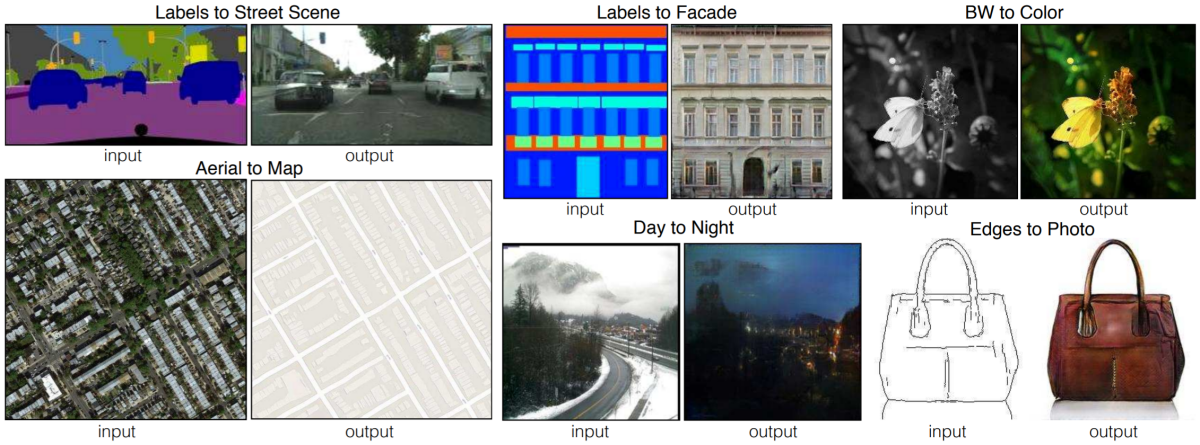
\includegraphics[width=\textwidth]{pix2pix.png}
    \caption{Image-to-image translation examples from~\cite{isola2017image}.}
    \label{fig:pix2pix}
\end{figure}

Recently, generative adversarial nets (GANs)~\cite{goodfellow2014generative} 
was 
introduced as an unsupervised learning method that can generatively model an 
unknown distribution. 
For a probabilistic distribution $f$ with support set $\mathcal{X}$, the 
objective of GAN is to find a generator $G:\mathbb{R}^n\rightarrow \mathcal{X}$ 
such that $G(Z)\sim f$, given $Z\sim \mathcal{N}(0,I_n)$. 
The goal is achieved by assuming a discriminator $D:\mathcal{X}\rightarrow 
{0,1}$ that discriminates a fake sample generated from $G$ against a real 
sample 
obtained from $f$. 
When parameterized as neural networks, both $G$ and $D$ can be trained by 
optimizing the min-max game: 
\begin{equation}
\min_G \max_D \mathbb{E}_{x\sim f}[\log D(x)] + \mathbb{E}_{x\sim G(Z)}[\log 
(1-D(x))]
\end{equation}
through gradient descent.
After convergence, $G(Z)$ should be identical to $f$, and $D$ will output $1/2$ 
everywhere, failing to discriminated fake samples from true samples. 

Conditional GANs~\cite{mirza2014conditional} was later introduced as an 
extension of the original GAN and forms the basis of image-to-image 
translation~\cite{isola2017image}. 
The idea is to extend the loss function in min-max game with a 
\textit{condition}, denoted as $y$: 
\begin{equation}
\min_G \max_D \mathbb{E}_{x\sim f}[\log D(x|y)] + \mathbb{E}_{x\sim 
G(Z|y)}[\log (1-D(x|y))]. 
\end{equation}
The condition can have many possible forms.
When $y$ represent the class label of an image (e.g., cats, dogs, horses, 
etc.), 
the generator is trained to generate images of a particular class. 
When $y$ represents an image, the generator is trained to modify the 
\textit{conditioning image} and match the \textit{target image} from $f$. 

Figure~\ref{fig:pix2pix} shows image-to-image translation examples 
from~\cite{isola2017image}. Conditioning images can be segmentation 
information, black-and-white photos or object edges. Target images can be real 
images with detail texture, colored photos, or object paints. Notice that there 
is no magic in this image-to-image translation.
All the missing information in translation are filled by a neural network 
trained a dataset containing thousands of image \textit{pairs}. 
The neural net learns by analyzing the difference between each pair of images.
Each type of translation is trained on a separate neural network and a 
separated 
dataset, and each neural network works like a ``domain expert'' that can only 
translate one type of images. 

